The  following Python code generates Fig. \ref{fig:tri_geo_8_tri_sss_py}
%
\begin{lstlisting}
codes/triangle.py
\end{lstlisting}
From the given information, 
%$\triangle ABC$ are 
\begin{align}
\label{eq:tri_geo_8_constr_a}
\vec{A} &= \myvec{4\\-6} 
\\
\vec{B} &= \myvec{3\\-2}, 
\label{eq:tri_geo_8_constr_b}
\\
\vec{C} &= \myvec{5\\2}
\label{eq:tri_geo_8_constr_c}
\end{align}
$\because \vec{M}$ is the midpoint of $AB$,
\begin{align}
\vec{M}= \frac{\vec{A}+\vec{B}}{2} = \frac{1}{2}\myvec{7\\-8}
\label{eq:tri_geo_8_constr_m}
\end{align}

$\because \vec{N}$ is the midpoint of $BC$,
\begin{align}
\vec{N}= \frac{\vec{B}+\vec{C}}{2} = \frac{1}{2}\myvec{8\\0}
\label{eq:tri_geo_8_constr_n}
\end{align}

$\because \vec{P}$ is the midpoint of $CA$,
\begin{align}
\vec{P}= \frac{\vec{C}+\vec{A}}{2} = \frac{1}{2}\myvec{9\\-4}
\label{eq:tri_geo_8_constr_p}
\end{align}
%%% Area of ABC
%If \textbf{S} is the semi-perimeter of $\triangle ABC$ then,\\
%$\textbf{S}= \frac{a+b+c}{2}$\\
%\text{or, } \textbf{S} = 8.325\\
%The area of $ \triangle ABC $,\\
%$\textbf{Area} = \sqrt{S(S-a)(S-b)(S-c)}$\\
%\text{or, } \textbf{Area} = 5.98\\

The  following Python code verifies the determinant values.

\begin{lstlisting}
codes/determinant_check.py
\end{lstlisting}

\begin{figure}[!ht]
\centering
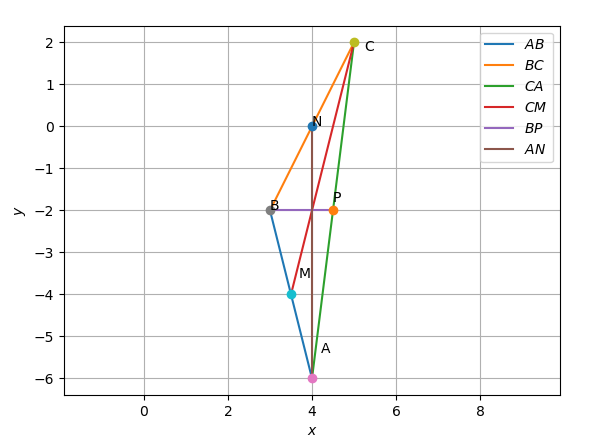
\includegraphics[width=\columnwidth]{./solutions/8/figs/triangle.eps}
\caption{}
\label{fig:tri_geo_8_tri_sss_py}
\end{figure}
For  $ \triangle ABC $ , the vertices are \textbf{A} , \textbf{B} and \textbf{C}.
So the area of the triangle $ \triangle ABC $  by using determinant will be :
\begin{equation}
\begin{aligned}
    Area = \frac{1}{2}\begin{vmatrix}
      4       & -6    & 1 \\ 
      3       & -2    & 1 \\
      5       & 2     & 1 \\
      
    \end{vmatrix} \xleftrightarrow[]{C_2\leftarrow \frac{C_2}{2}} \frac{2}{2}\begin{vmatrix}
      4       &-3    & 1 \\ 
      3       &-1    & 1 \\
      5       & 1    & 1 \\
      
    \end{vmatrix}\\
    \xleftrightarrow[R_3 \leftarrow R_3-R_1]{R_2\leftarrow R_2-R_1}
    \begin{vmatrix}
      4       & -3    & 1 \\ 
      -1       & 2    & 0 \\
      1       & 4   & 0 \\
      
    \end{vmatrix}  \xleftrightarrow[]{R_3\leftarrow R_3+R_2}
    \begin{vmatrix}
      4       & -3    & 1 \\ 
      -1       & 2    & 0 \\
      0       & 6   & 0 \\
      
    \end{vmatrix} \\ \xleftrightarrow[]{R_3\leftarrow \frac{R_3}{6}}
    6 \begin{vmatrix}
      4       & -3    & 1 \\ 
      -1       & 2    & 0 \\
      0       & 1   & 0 \\
      
    \end{vmatrix} \\
    =-6
   \end{aligned}
  \end{equation}
Now, we will consider the absolute value of area only. So, $Area$ = $\abs{-6}$ = 6.\\
To verify the problem statement we have to check 3 cases:\\
 %%% Area of ABP
\textbf{Case 1:} When \textbf{BP} is median, we will consider $ \triangle ABP $ triangle. In that case, the vertices will be \textbf{A}, \textbf{B} and \textbf{P}.\\
Now, the area of $ \triangle ABP $ will be :\\
%the length of \textbf{BP} (x1)= $\norm{\textbf{B}-\textbf{P}}$= 1.5\\
%the length of \textbf{AP} (x2)= $\norm{\textbf{A}-\textbf{P}}$= 4.03\\
%The semi-perimeter of the triangle $ \triangle ABP $ is \textbf{S1}.\\
%$\textbf{S1}= \frac{x1+x2+c}{2}$\\
%\text{or, } \textbf{S1} = 4.825\\
%The area of $ \triangle ABP $,\\
%$\textbf{A1} = \sqrt{S1(S1-x1)(S1-x2)(S1-c)}$\\
%\text{or, } \textbf{A1} = 2.987\\
\begin{equation}
\begin{aligned}
    A1 = \frac{1}{2}\begin{vmatrix}
      4       & -6    & 1 \\ 
      3       & -2    & 1 \\
      4.5       & -2     & 1 \\
      
    \end{vmatrix} \xleftrightarrow[]{C_2\leftarrow \frac{C_2}{(-2)}} \frac{(-2)}{2}\begin{vmatrix}
      4       &3    & 1 \\ 
      3       &1    & 1 \\
      4.5       & 1    & 1 \\
      
    \end{vmatrix}\\
    \xleftrightarrow[R_3 \leftarrow R_3-R_1]{R_2\leftarrow R_2-R_1}
    (-1)\begin{vmatrix}
      4       & 3    & 1 \\ 
      -1       & -2    & 0 \\
      0.5       & -2   & 0 \\
      
    \end{vmatrix} \\ \xleftrightarrow[]{R_3 \leftarrow R_3-R_2}
    (-1)\begin{vmatrix}
      4       & 3    & 1 \\ 
      -1       & -2    & 0 \\
      1.5       & 0   & 0 \\
      
    \end{vmatrix}\\
    =-3
   \end{aligned}
  \end{equation}
But, we will consider the absolute value of area only. So, \textbf{A1} = $\abs{-3}$ = 3.\\
\text{or, } \textbf{A1} = $\frac{1}{2}$(Area of $\triangle ABC$)\\
%%% Area of ABN
\textbf{Case 2:} When \textbf{AN} is median,we will consider $ \triangle ABN $ triangle. In that case, the vertices will be \textbf{A}, \textbf{B} and \textbf{N}.\\
Now, the area of $ \triangle ABN $ will be :\\
%For $ \triangle ABN $ ,\\
%the length of \textbf{AN} (y1)= $\norm{\textbf{A}-\textbf{N}}$= 6\\
%the length of \textbf{BN} (y2)= $\norm{\textbf{B}-\textbf{N}}$= 2.24\\
%The semi-perimeter of the triangle $ \triangle ABN $ is \textbf{S2}.\\
%$\textbf{S2}= \frac{y1+y2+c}{2}$\\
%\text{or, } \textbf{S2} = 6.18\\
%The area of $ \triangle ABN $,\\
%$\textbf{A2} = \sqrt{S2(S2-y1)(S2-y2)(S2-c)}$\\
%\text{or, } \textbf{A2} = 2.99\\
\begin{equation}
\begin{aligned}
    A2 = \frac{1}{2}\begin{vmatrix}
      4       & -6    & 1 \\ 
      3       & -2    & 1 \\
      4       & 0     & 1 \\
      
    \end{vmatrix} \xleftrightarrow[]{C_2\leftarrow \frac{C_2}{(-2)}} \frac{(-2)}{2}\begin{vmatrix}
      4       &3    & 1 \\ 
      3       &1    & 1 \\
      4       & 0    & 1 \\
      
    \end{vmatrix}\\
    \xleftrightarrow[R_3 \leftarrow R_3-R_1]{R_2\leftarrow R_2-R_1}
    (-1)\begin{vmatrix}
      4       & 3    & 1 \\ 
      -1       & -2    & 0 \\
      0       & -3   & 0 \\
      
    \end{vmatrix} \\ \xleftrightarrow[]{R_3 \leftarrow \frac{R_3}{(-3)}}
    3 \begin{vmatrix}
      4       & 3    & 1 \\ 
      -1       & -2    & 0 \\
      0       & 1   & 0 \\
      
    \end{vmatrix}\\
    =-3
   \end{aligned}
  \end{equation}
But, we will consider the absolute value of area only. So, \textbf{A2} = $\abs{-3}$ = 3.\\
\text{or, } \textbf{A2} = $\frac{1}{2}$(Area of $\triangle ABC$)\\
%%% Area of CAM
\textbf{Case 3:} When \textbf{CM} is median,we will consider $ \triangle CAM $ triangle. In that case, the vertices will be \textbf{A}, \textbf{C} and \textbf{M}.\\
Now, the area of $ \triangle CAM $ will be :\\
%the length of \textbf{CM} (z1)= $\norm{\textbf{C}-\textbf{M}}$= 6.18\\
%the length of \textbf{AM} (z2)= $\norm{\textbf{A}-\textbf{M}}$= 2.06\\
%The semi-perimeter of the triangle $ \triangle CAM $ is \textbf{S3}.\\
%$\textbf{S3}= \frac{z1+z2+b}{2}$\\
%\text{or, } \textbf{S3} = 8.15\\
%The area of $ \triangle CAM $,\\
%$\textbf{A3} = \sqrt{S3(S3-z1)(S3-z2)(S3-b)}$\\
%\text{or, } \textbf{A3} = 2.96\\
\begin{equation}
\begin{aligned}
    A3 = \frac{1}{2}\begin{vmatrix}
      5       & 2    & 1 \\ 
      4       & -6    & 1 \\
      3.5       & -4     & 1 \\
      
    \end{vmatrix} \xleftrightarrow[]{C_2\leftarrow \frac{C_2}{2}} \frac{2}{2}\begin{vmatrix}
      5       &1    & 1 \\ 
      4       &-3    & 1 \\
      3.5       & -2    & 1 \\
      
    \end{vmatrix}\\
    \xleftrightarrow[R_3 \leftarrow R_3-R_1]{R_2\leftarrow R_2-R_1}
    \begin{vmatrix}
      5       & 1    & 1 \\ 
      -1       & -4    & 0 \\
      -1.5       & -3   & 0 \\
      
    \end{vmatrix} \\ \xleftrightarrow[R_3 \leftarrow \frac{R_3}{(-1.5)}]{R_2 \leftarrow \frac{R_2}{(-1)}}
    1.5 \begin{vmatrix}
      5       & 1    & 1 \\ 
      1       & 4    & 0 \\
      1       & 2   & 0 \\
      
    \end{vmatrix}\\ \xleftrightarrow[]{R_3\leftarrow R_3-R_2}
    1.5 \begin{vmatrix}
      5       & 1    & 1 \\ 
      1       & 4    & 0 \\
      0       & -2   & 0 \\
      
    \end{vmatrix}\\
    =-3
   \end{aligned}
  \end{equation}
But, we will consider the absolute value of area only. So, \textbf{A3} = $\abs{-3}$ = 3.\\
\text{or, } \textbf{A3} = $\frac{1}{2}$(Area of $\triangle ABC$)\\

Hence, the above problem statement is verified. 
%Besides this, the above problem statement is also verified by using python code: $codes/determinant-check.py$



